\documentclass[hidelinks, 12pt, oneside]{article}
\usepackage{bookmark}
\usepackage{graphicx}
\usepackage{hyperref}
\usepackage{titlesec}
\setcounter{secnumdepth}{4}
\usepackage[utf8]{inputenc}
\usepackage[english]{babel}


\begin{document}
	\begin{center}
    \centering
    
%University logo
    
\includegraphics[width=144px]{img/icon.png}
    \rule{0\linewidth}{0.15\linewidth}\par
    
    		\begin{center}
		{\uppercase{\Large User Manual\par}}
   		{\Large iCrawler \par}
   			\vspace{1cm} 
   		{\Large Emilio Mumba  \par} 
    		\vspace{1cm}
		   		
    		{\Large The 5 Concurrent Nodes \par} 
    		\vspace{1cm}
		
		{\normalsize Khathutshelo Shaun Matidza\par}
		{\normalsize Sylvester Sandile Mpangane\par}
		{\normalsize Thabang Michael Letageng\par}
		{\normalsize Matthew Nel\par}
		
		\end{center}

		\textbf{}		
		\centering
		\vspace{2cm}
		Department of Computer Science, University of Pretoria

		
	 	{\Large  September 2015}
\end{center}
\clearpage


	\tableofcontents
	
	\newpage
	\section{Vision and Scope}
		\subsection{Project Vision}
		\vspace{0.3 cm}
	  	Digital forensics is defined as the use of scientifically derived and proven methods towards the preservation, 			collection, validation, identification, analysis, interpretation and presentation of digital evidence derived 			from digital sources for the sole purpose of facilitating or furthering the reconstruction of events found to 			be criminal or helping to anticipate the unauthorized actions shown to be disruptive to planned operations.
		Readiness is considered as the process of being prepared for a digital investigation before an incident has 			occurred. \\\\
		The proposal of a mobile monitoring application will promote readiness in digital forensics and protect mobile 			users from malicious entities and activities. It aims to provide a proactive measure that is undertaking by the 		mobile device user or mobile device owner. Having this application installed on mobile devices will proactively 		ensure that relevant digital evidence is made ready and available before an incident occurs. The mobile 				monitoring application is expected to monitor user activities on a mobile device and report application data/			logs to a dashboard on a desktop computer. It will generate reports giving the investigator quick and 					comprehensive data/logs that provide a starting point during a mobile device investigation. \newline\newline
		The objective of the mobile monitoring application is to collect data/logs and assist in understanding the 				activities performed by a mobile user as well as shedding more light into the behaviour of the mobile user. 			Combining activities from the various applications promotes a proactive approach which in turn enforces 				proactive (readiness) measures.
		
		\newpage
		\subsection{Project Scope}	
		The high level modules of the iCrawler monitoring app is as indicated on the figure below. The responsibilities 			of each module are also noted.
		
			\begin{figure}[!htbp]
    			\centering
    			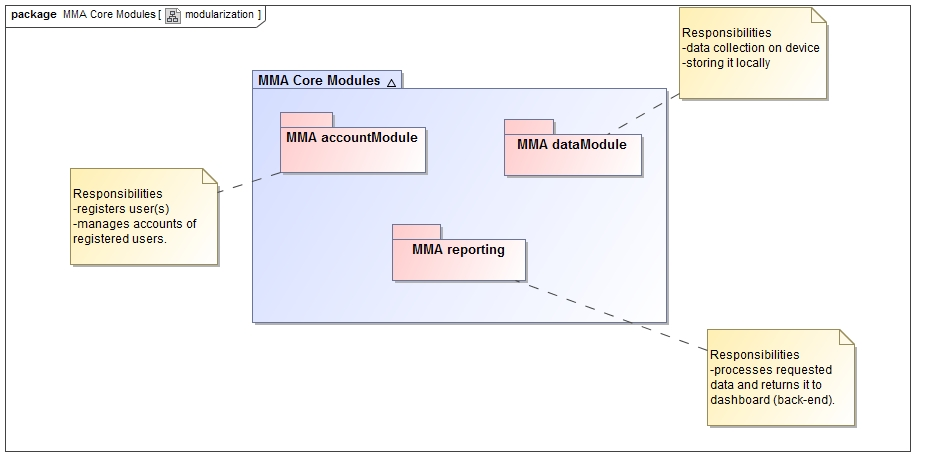
\includegraphics[width=0.9\textwidth]{img/highLevelSystem.jpg}
    			\caption{High Level App Modules}
    			\label{fig:highLevelSystem}
			\end{figure}


	\section{Application Requirements and Design}
	The following section will explain each module in the mobile monitoring app. The use-case design, functional requirements extracted from the use-case along with the selected service contracts will also be discussed.\newline
	
	\subsection{Modular System}
	 The application uses modular design approach. This allows the following to be achieved:
	 \begin{itemize}
	\item add new functionality in the future
 	\item decouple the system
	\end{itemize}


	
	\subsection{iCrawler - Account Module}
	%You will have to elaborate on what the module does (look at the high level module notes for help)
	\subsubsection{Scope}
	%The width and height of the image should not be changed. Just uncomment the line below and specify img source
	
	\begin{figure}[!htbp]
    		\centering
    		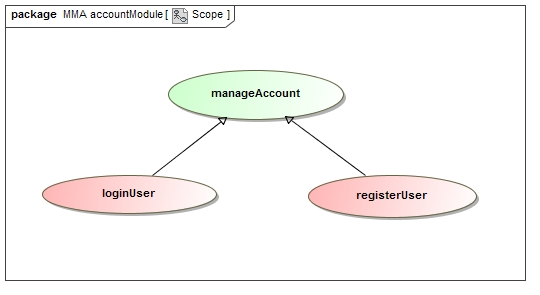
\includegraphics[width=0.9\textwidth]{img/scopeAccounts.jpg}
    		\caption{Scope - mmaAccounts module}
    		\label{fig:accountsScope}
		\end{figure}
		
	\subsubsection{Use-Cases}
		This section provides details on the use-case requirements for the use-cases offered by this module.
	\paragraph{registerUser - priority: important}
		This use-case registers a user on initial installation after user accepts terms and conditions of use.
	
	\newpage
	\subparagraph{Service Contract:}
		The service contract for registerUser is shown in the figure below. The pre-conditions are enforced (raises an exception if not met) and on
		success the user is registered and the device and user data is persisted to the database.
		
		\begin{figure}[!htbp]
    		\centering
    		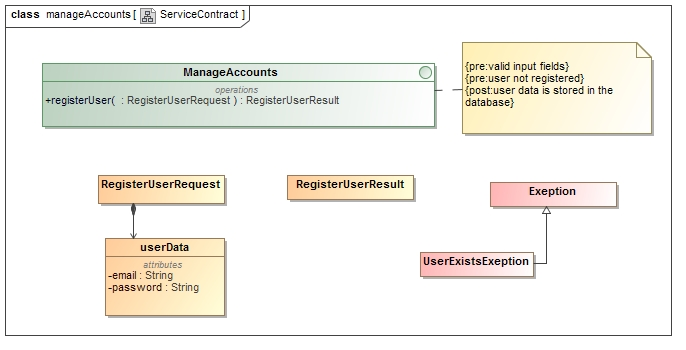
\includegraphics[width=0.9\textwidth]{img/serviceContractRegisterUser.jpg}
    		\caption{Service Contract - Register user}
    		\label{fig:ServiceCon_registerUser}
		\end{figure}
		
		
		\begin{figure}[!htbp]
    		\centering
    		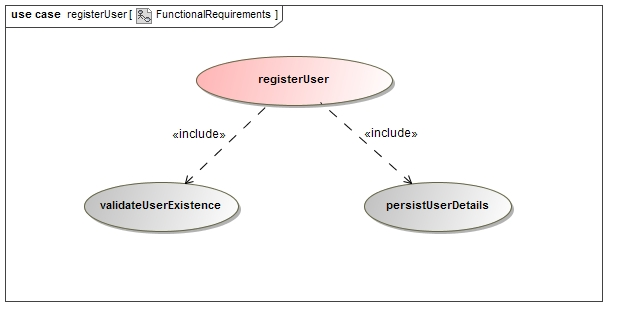
\includegraphics[width=0.9\textwidth]{img/functionalRequirementsRegister.jpg}
    		\caption{Functional Requirements - Register user}
    		\label{fig:FunctionalReq_registerUser}
		\end{figure}
		
		
		
		\paragraph{Process specification:}		
		When a request is made for a user to register, a connection to the database must be established. If no connection to the database can be made then an exception is thrown. Alternatively, validateUserExistance is called to check if that user exists or not. If the user does exist then an exception is thrown, if not then that user is registered.
		
		\begin{figure}[!htbp]
    		\centering
    		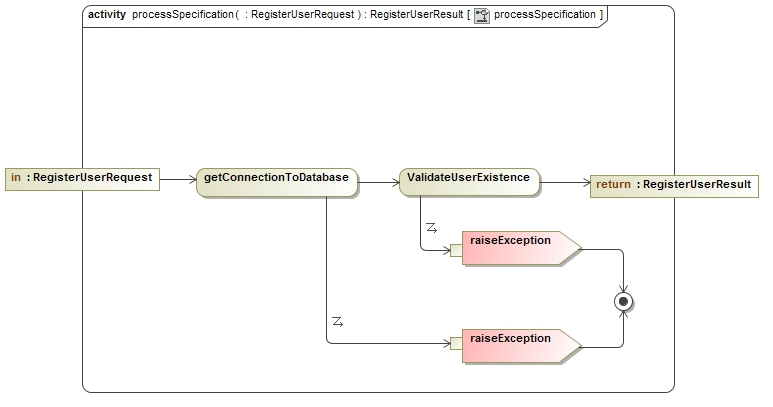
\includegraphics[width=0.9\textwidth]{img/processSpecificationRegisterUser.jpg}
    		\caption{Process Specification - Register user}
    		\label{fig:ProcessSpec_registerUser}
		\end{figure}
				
	
	\paragraph{loginUser - priority: important}
		This use-case logins a user on initial installation after user accepts terms and conditions of use.
		
	\subparagraph{Service Contract:}
		The service contract for loginUser is shown in the figure below. The pre-conditions that are enforced(raises and exception if not met) and on success the user is logged in and the device and user data is persisted to the database.\newline 	
	
		\begin{figure}[!htbp]
    		\centering
    		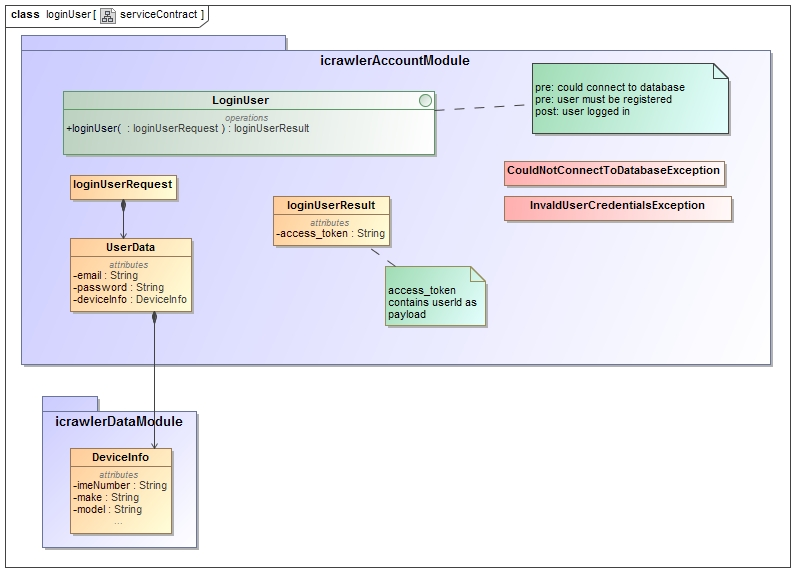
\includegraphics[width=0.9\textwidth]{img/serviceContractLoginUser.jpg}
    		\caption{Service Contract - Login user}
    		\label{fig:ServiceCon_loginUser}
		\end{figure}
		
		
		\begin{figure}[!htbp]
    		\centering
    		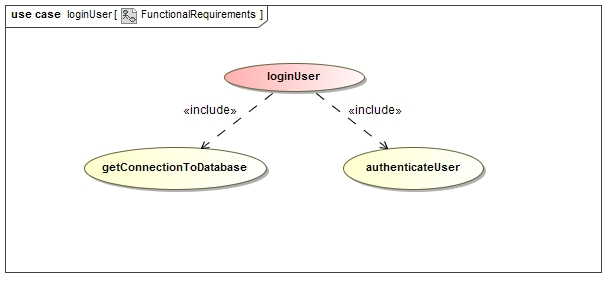
\includegraphics[width=0.9\textwidth]{img/functionalRequirementsLoginUser.jpg}
    		\caption{Functional Requirements - Login user}
    		\label{fig:FunctionalReq_loginUser}
		\end{figure}
		
				
		\newpage
		\paragraph{Process specification:}
		When a request is made for a user to login a connection to the database must be established. If no connection to the database can be made then an exception is thrown. If a connection to the database is established, a login request is made, if user credentials are valid	the user is logged in otherwise an exception is thrown.		
		
		
		\begin{figure}[!htbp]
    		\centering
    		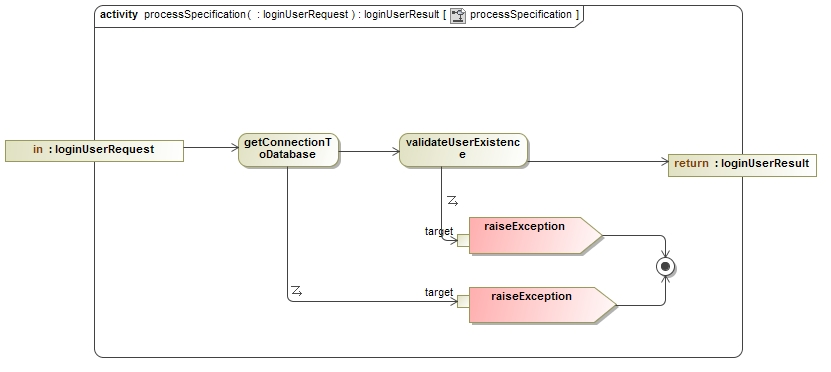
\includegraphics[width=0.9\textwidth]{img/processSpecificationLoginUser.jpg}
    		\caption{Process Specification - Login user}
    		\label{fig:ProcessSpec_loginUser}
		\end{figure}
		\newpage
		
		\subsubsection{Domain Model}
		The domain model for this module is very simple and straight forward.It only requires a valid service request.
		
		
		\begin{figure}[!htbp]
    		\centering
    		\includegraphics[width=0.9\textwidth]{img/DomainModelAccountModule.jpg}
    		\caption{Domain Model - Account Module}
    		\label{fig:DomainMod_accountModule}
		\end{figure}
		\newpage
				
		\subsubsection{Design Pattern}
		In order to depict the behavior of this module, we use a State design pattern. This highlights the transitions 
		between a user login and user register.
		
		\begin{figure}[!htbp]
    		\centering
    		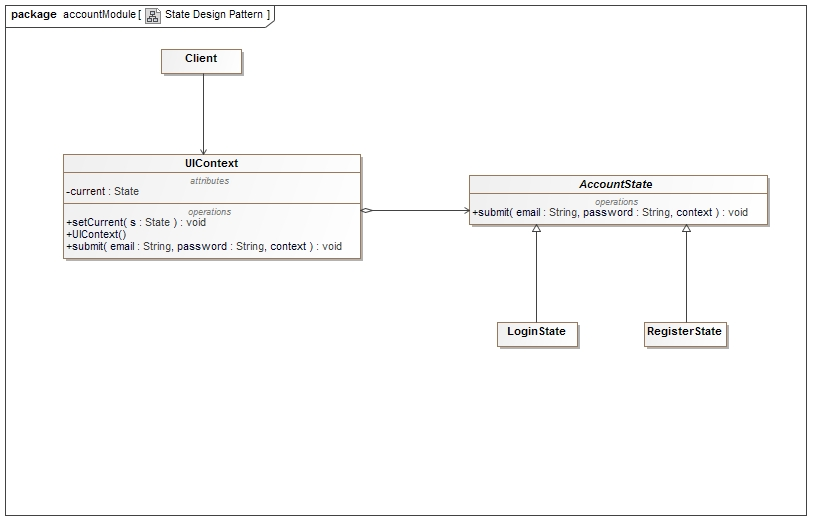
\includegraphics[width=0.9\textwidth]{img/design_patterns/AccountModule_StateDesignPattern.jpg}
    		\caption{Design Pattern - State}
    		\label{fig:DesignPat_state}
		\end{figure}
		\newpage
		
	\subsection{MobileMonitoringApp - Data module}
	%You will have to elaborate on what the module does (look at the high level module notes for help)
	\subsubsection{Scope}
	
		\begin{figure}[!htbp]
    		\centering
    		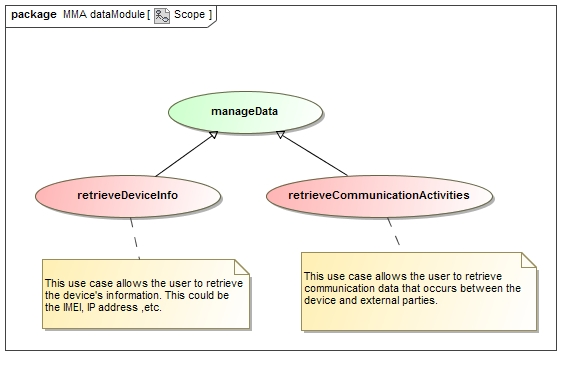
\includegraphics[width=0.9\textwidth]{img/scopeData.jpg}
    		\caption{Scope - dataModule}
    		\label{fig:Scope_dataModule}
		\end{figure}	
		
		
	\subsubsection{Use-Cases}
		This section provides details on the use-case requirements for the use-cases offered by this module.	
		
	\paragraph{retrieveDeviceInfo - priority: important}
		The retrieveDeviceInfo use case retrieves all the relevant device information from the device.\newline
		
		\subparagraph{Service Contract:}
		The service contract for retrieveDeviceInfo is shown in the figure below. The retrieveDeviceInfo 			receives a retrieveDeviceInfoRequest object that specifies the type of data to be retrieved and 			stored locally on to a database.
		
		
		\begin{figure}[!htbp]
    		\centering
    		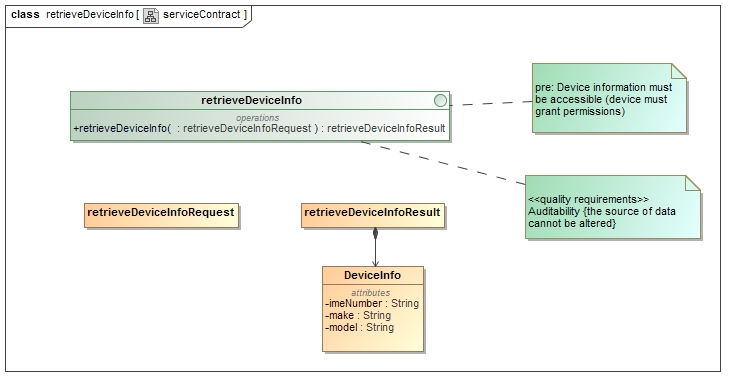
\includegraphics[width=0.9\textwidth]{img/serviceContractRetrieveDeviceInfo.jpg}
    		\caption{Service Contract - retrieveDeviceInfo}
    		\label{fig:ServiceCon_retrieveDeviceInfo}
		\end{figure}
				
		
		\begin{figure}[!htbp]
    		\centering
    		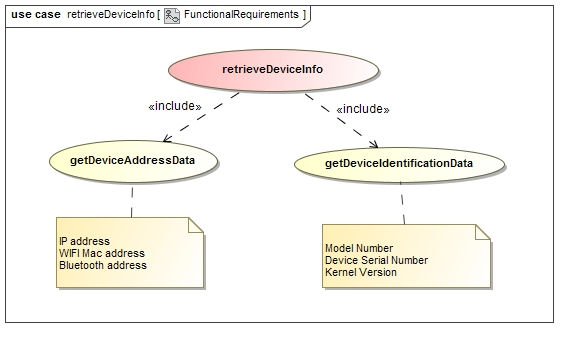
\includegraphics[width=0.9\textwidth]{img/functionalRequirementsRetrieveDeviceInfo.jpg}
    		\caption{Functional Requirements - retrieveDeviceInfo}
    		\label{fig:FunctionalReq_retrieveDeviceInfo}
		\end{figure}
		
		
		\paragraph{Process specification:}
		When a request is made for device data to be retrieved. The service checks for the type of data to 			be retrieved and follows the required channels to retrieve the data. If the service is not 					successful then an exception is raised. If the service is successful then an object with the 				required data is returned as a result of the query.
		
		\begin{figure}[!htbp]
    		\centering
    		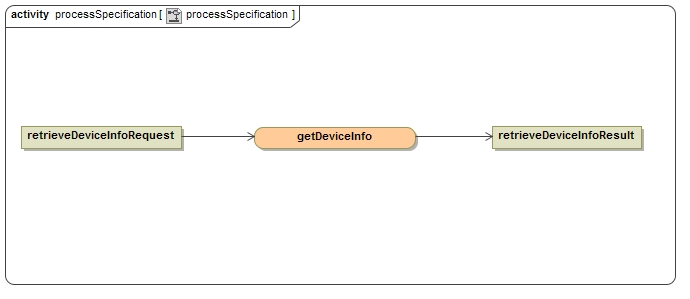
\includegraphics[width=0.9\textwidth]{img/processSpecificationRetrieveDeviceInfo.jpg}
    		\caption{Process Specification - retrieveDeviceInfo}
    		\label{fig:ProcessSpec_retrieveDeviceInfo}
		\end{figure}
		
		
		\paragraph{retrieveCommunicationActivities - priority: important}
		The retrieveCommunicationAcitivites use-case retrieves all the users communication activities from 		the various apps on the device.\newpage
		
		\subparagraph{Service Contract:}
		The service contract for retrieveCommunicationAcitivites is shown in the figure below. The 					retrieveCommunicationActivitiesRequest requests the data regardless of the data type and 		retrieveCommunicationActivitiesRequest retrieves the data where it packages the data and stores it on the database locally.
		
		\begin{figure}[!htbp]
    		\centering
    		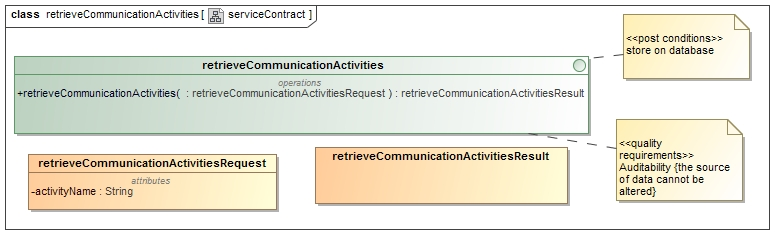
\includegraphics[width=0.9\textwidth]{img/serviceContractRetrieveCommunicationActivities.jpg}
    		\caption{Service Contract - retrieveCommunicationAcitivites}
    		\label{fig:ServiceCon_retrieveCommunicationAcitivites}
		\end{figure}
				

		\begin{figure}[!htbp]
    		\centering
    		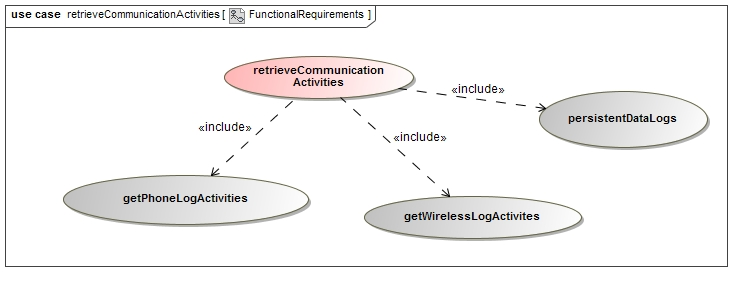
\includegraphics[width=0.9\textwidth]{img/functionalRequirementsRetrieveCommunicationActivities.jpg}
    		\caption{Functional Requirements - Retrieve Communication Acitivites}
    		\label{fig:FunctionalReq_retrieveCommunicationAcitivites}
		\end{figure}	
		
		
			\newpage
			\paragraph{Process specification:}
			The  service receives a request that specifies the type of activity the service needs to collect data from.The service will retrieve the data from that activity and if it fails then an exception will be raised.The result from the function will be an object that wraps the required data.
			
			
			\begin{figure}[!htbp]
    		\centering
    		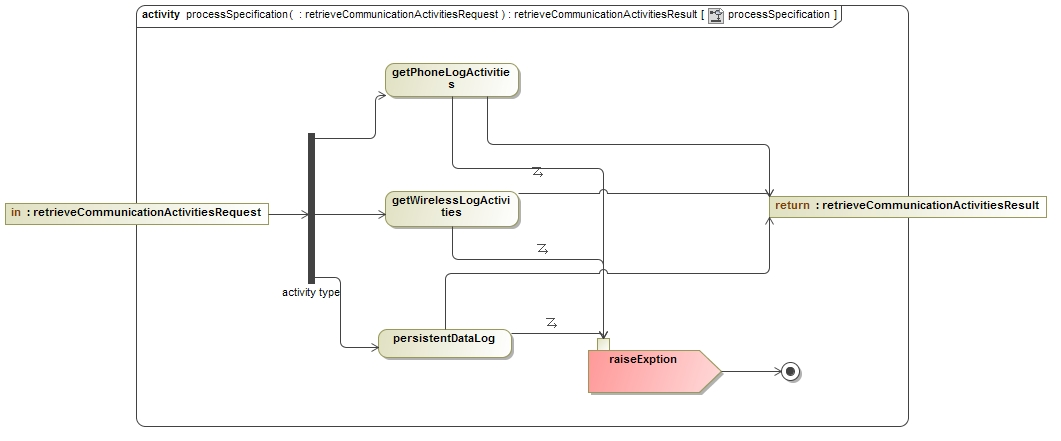
\includegraphics[width=0.9\textwidth]{img/processSpecificationRetrieveCommunicationActivities.jpg}
    		\caption{Process Specification - Retrieve Communication Acitivites}
    		\label{fig:ProcessSpec_retrieveCommunicationAcitivites}
		\end{figure}
		\newpage
	
		\subsubsection{Domain Model}
		The domain model for this module is very simple and straight forward.It only requires a valid service request.
		
		
		\begin{figure}[!htbp]
    		\centering
    		\includegraphics[width=0.9\textwidth]{img/DomainModelDataModule.jpg}
    		\caption{Domain Model - Data Module}
    		\label{fig:DomainMod_dataModule}
		\end{figure}
		\newpage
		
	\subsection{MobileMonitoringApp - Reports module}
	%You will have to elaborate on what the module does (look at the high level module notes for help)
	\subsubsection{Scope}
	
	
	\begin{figure}[!htbp]
    		\centering
    		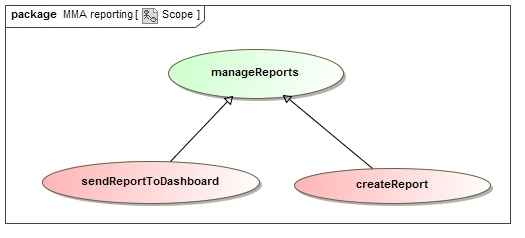
\includegraphics[width=0.9\textwidth]{img/scopeReports.jpg}
    		\caption{Scope - Reporting Module}
    		\label{fig:Scope_reportingModule}
		\end{figure}
			
		
	\subsubsection{Use-Cases}
			This section provides details on the use-case requirements for the use-cases offered by this module.
		\paragraph{ createReport - priority: important}
		This use-case retrieves logs from the device and creates a report from those specific logs.
		\newpage
		
		\subparagraph{Service Contract:}
					The service create report is shown in the figure below. The pre-condition is enforced. 
					
				
		\begin{figure}[!htbp]
    		\centering
    		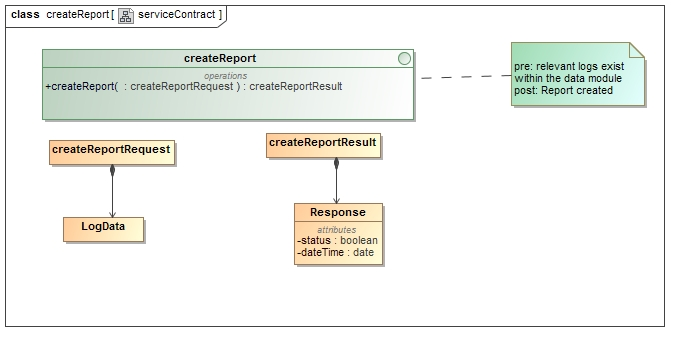
\includegraphics[width=0.9\textwidth]{img/serviceContractcreateReport.jpg}
    		\caption{Service Contract - Create Report}
    		\label{fig:ServiceCon_createReport}
		\end{figure}
		
		
		\begin{figure}[!htbp]
    		\centering
    		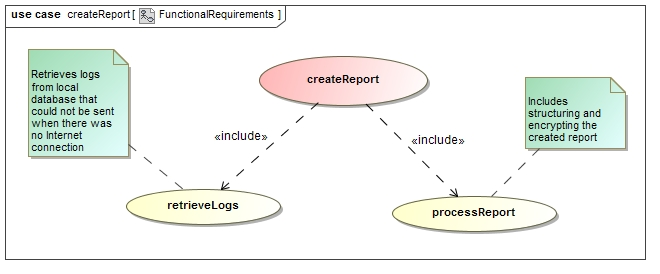
\includegraphics[width=0.9\textwidth]{img/FunctionalRequirementscreateReport.jpg}
    		\caption{Functional Requirements - Create Report}
    		\label{fig:FunctionalReq_createReport}
		\end{figure}
		
		
		\begin{figure}[!htbp]
    		\centering
    		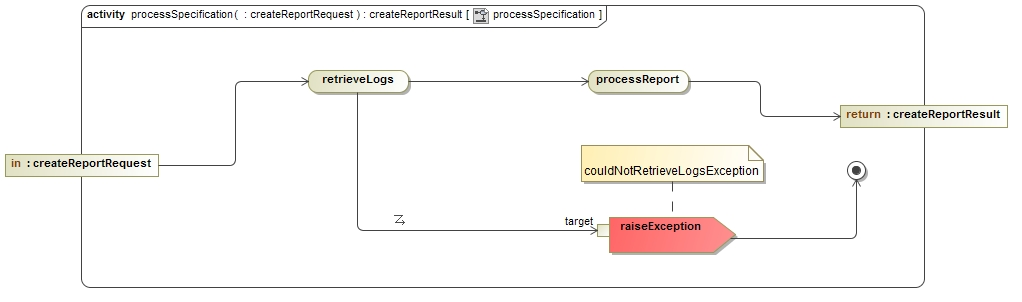
\includegraphics[width=0.9\textwidth]{img/processSpecificationcreateReport.jpg}
    		\caption{Process Specification - Create Report}
    		\label{fig:ProcessSpec_createReport}
		\end{figure}
		\newpage			
					
								
		\paragraph{ sendReportToDashboard - priority: important}
		This module sends the report onto a server where they will be saved on a database to de displayed later on a dashboard .\newline
		\subparagraph{Service Contract:}
			The service contract for sendReportToDashboard is shown in the figure below. The pre-condition is not enforced i.e. If the app fails to establish a connection with the server, the report will be saved temporarily on the device until a connection is established.
			
		
		\begin{figure}[!htbp]
    		\centering
    		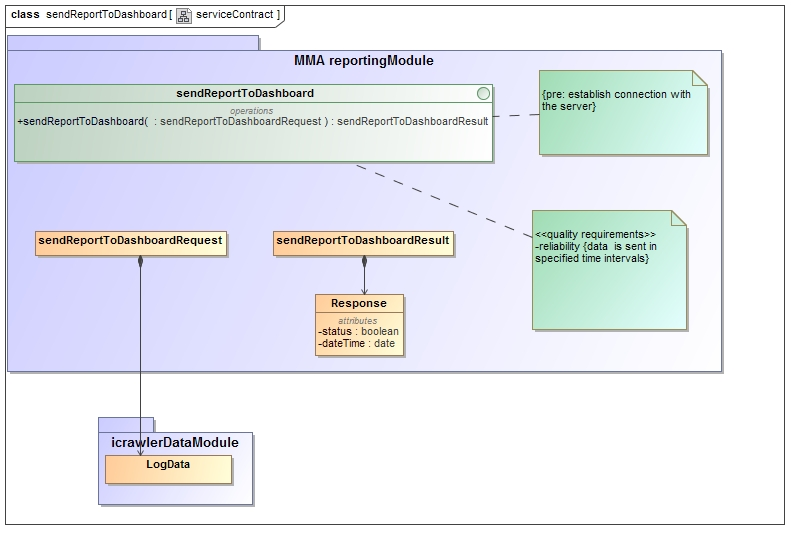
\includegraphics[width=0.9\textwidth]{img/serviceContractSendReportToDashboard.jpg}
    		\caption{Service Contract - Send Report To Dashboard}
    		\label{fig:ServiceCon_submitReport}
		\end{figure}
		\newpage	
			
		\begin{figure}[!htbp]
    		\centering
    		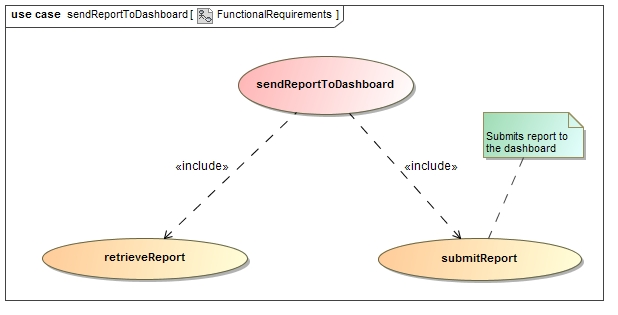
\includegraphics[width=0.9\textwidth]{img/functionalRequirementsSendReportToDashboard.jpg}
    		\caption{Functional Requirements - Send Report To Dashboard}
    		\label{fig:FunctionalReq_submitReport}
		\end{figure}
		
		
		\begin{figure}[!htbp]
    		\centering
    		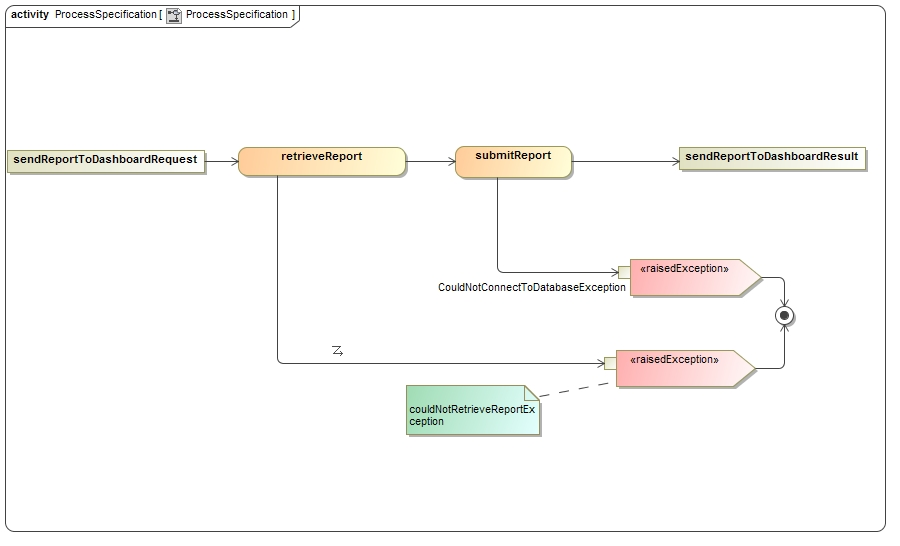
\includegraphics[width=0.9\textwidth]{img/ProcessSpecificationSendResportToDashboard.jpg}
    		\caption{Process Specification - Send Report To Dashboard}
    		\label{fig:ProcessSpec_submitReport}
		\end{figure}
		\newpage
		
			\paragraph{Domain Model:}
			This section contains the domain model for the reporting module. This module retrieves logs from the data module. 
			
			
			\begin{figure}[!htbp]
    		\centering
    		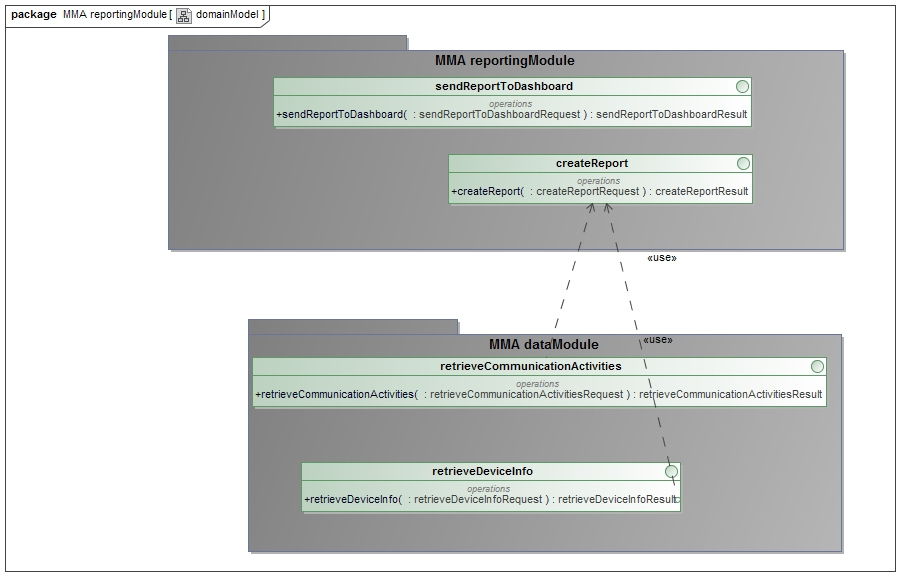
\includegraphics[width=0.9\textwidth]{img/domainModelReportModule.jpg}
    		\caption{Domain Model - mmaReporting Module}
    		\label{fig:DomainModel_reportingModule}
		\end{figure}	
\end{document}
